\section{\added[id=1010]{Resolution of the dispersion equation using a domain decomposition method}}
\label{sec:DDM}

\indent \added[id=2017]{We propose in this section a DDM for solving the problem }

\begin{equation}
	\label{eq:problemMonodomainContinuous}
	\begin{cases}
	u_t + u_{xxx} = 0, \ \ x \in \Omega, \ \  t \geq t_0 \\
	u(t_0,x) = u^{exact}(t_0,x) , \ \ x \in \Omega \\ 
	\Upsilon_1(u,-L) = 0, \ \ t \geq t_0 \\
	\Upsilon_2(u,L) = 0, \ \ t \geq t_0 \\
	\Upsilon_3(u,L) = 0, \ \ t \geq t_0
	\end{cases}
\end{equation}

\noindent \added[id=2017]{in the domain  $\Omega=[a,b]$}.

\indent \added[id=1010]{We firstly present a brief review of the DDM considered here, the parallel or additive Schwarz method (ASM) and then we propose IBCs for applying it to the problem solved in this paper.}

\indent \deleted[id=2017]{The operators \eqref{eq:appDiscTBCP0} derived in the previous section will be applied as interface boundary conditions (IBC) in a domain decomposition method (DDM). Firstly, following \cite{Japhet2003},we describe the DDM considered here, and after we describe and test the incorporation of the proposed IBCs.}

\subsection{The Schwarz Method}

\indent \replaced[id=1010]{Domain decomposition methods}{ DDMS} allow to decompose a domain $\Omega$ in multiple subdomains $\Omega_i$ (that can possibly overlap) and solve the problem in each one of them. Therefore, one must find functions that satisfy the PDE in each subdomain and that match on the interfaces. 

\indent \added[id=1010]{The first DDM developed was the \added[id=1010]{alternating or multiplicative} Schwarz method, in which the IBCs for computing the solution in a subdomain are function of the most updated solution in the neighbor subdomains. We consider here a modified version of this algorithm, introduced more recently by \cite{Lions1988} and known as parallel or additive Schwarz method. In this algorithm, the IBCs for computing the solution $u_i^k$, in the subdomain $\Omega_i$ and iteration $k$, are always constructed using the solution $u_j^{k-1}, \ \ j \neq i$, of the previous iteration in the neighbor subdomains.}

\indent \added[id=1010]{This modification originates an inherently parallel algorithm, which one naturally implements with parallel computing. The advantages obtained with the parallelism become more evident when the number of subdomains increases \cite{Lions1988}.}

\indent \added[id=1010]{In the ASM, the boundary condition for the problem in $\Omega_i$, in each interface between the subdomains $\Omega_i$ and $\Omega_j$, can be written as}

\begin{equation}
	\label{eq:genericIBC}
\mathcal{B}_i(u_i^{k+1}) = \mathcal{B}_i(u_j^{k})
\end{equation}

\noindent \added[id=1010]{where \eqref{eq:genericIBC}, $\mathcal{B}_i$ denotes the operator of the IBC. This operator allows the construction of more general Schwarz methods: in the original one, the IBCs are Dirichlet conditions (\emph{i.e.}, $\mathcal{B}_i(u) = u$  ) \cite{Japhet2003,Lions1990}.}

\indent Without loss of generality, in the following we consider a domain $\Omega$ decomposed in two non-overlapping subdomains, $\Omega_1$ and $\Omega_2$, with $\Gamma = \Omega_1 \bigcap \Omega_2$.

\indent When implementing a Schwarz method, one must define appropriate operators $\mathcal{B}_i$ such that:

\begin{itemize}
\begingroup \item There is a unique solution $u_i$ in each subdomain $\Omega_i$; \endgroup
\item The solution $u_i$ in each subdomain $\Omega_i$ converges to $u|_{\Omega_i}$, \emph{i.e.}, the solution $u$, restricted to $\Omega_i$, of the problem in the monodomain $\Omega$;
\end{itemize} 

\indent Moreover, one wants the method to show a fast convergence.

\indent In fact, accordingly to \cite{Japhet2003}, the optimal additive Schwarz method for solving the problem 

\begin{equation*}
\begin{cases}
\mathcal{A}(u) = f \ \ \text{in} \ \ \Omega\\
u = 0 \ \ \text{on} \ \ \partial\Omega\\
\end{cases}
\end{equation*}

\noindent where $\mathcal{A}$ is a partial differential operator, is the one which uses as IBCs the exact TBCs for the problem, which are given by

$$\mathcal{B}_i(u) = \frac{\partial}{\partial n_i}u + D2N(u)$$

\noindent where $\partial n_i$ is the outward normal to $\Omega_i$ on $\Gamma$ , and the $D2N$ (Dirichlet to Neumann) operator is defined by

$$\left. D2N : \alpha(x) \mapsto \frac{\partial}{\partial n_i^c}v \right\rvert_\Gamma$$

\noindent with $\alpha$ defined on $\Gamma$. $v$ is solution of the following problem, solved in the complementary set of $\Omega_i$, denoted by $\Omega_i^c$

\begin{equation*}
\begin{cases}
\mathcal{A}(v) = f \ \ \text{in} \ \ \Omega_i^c\\
v = 0 \ \ \text{on} \ \ \partial \Omega_i \backslash \Gamma \\
v = \alpha \ \ \text{on} \ \ \Gamma
\end{cases}
\end{equation*}

\indent The ASM using such exact TBCs is optimal in the sense that it converges in two iterations, and no other ASM can converge faster \cite{Japhet2003}. Nevertheless, these TBCs, in general, are not simple to compute both analytically and numerically. More specifically, they are nonlocal in time, so they must be approximated for an efficient numerical implementation \cite{Xavieretal2008}. \added[id=2017]{These facts motivate us to look for simpler operators to use as IBCs in the ASM. We propose them based on the exact TBCs operators for the equation \eqref{eq:DKdV}, as derived by} \cite{besse2015}.  \deleted[id=2017]{These facts motivate us to implement the operators \eqref{eq:appDiscTBCP0} as interface boundary conditions for the ASM: they were derived based on the exact TBCs for the equation \eqref{eq:DKdV}, but, on the other hand, they are very simple to compute.}

\subsection{\added[id=2017]{Interface boundary condition operators based on the exact TBCs for the dispersion equation}}
\label{sec:TBC}

\indent In \cite{besse2015}, TBCs are derived for the one-dimensional continuous linearized KdV equation (or Airy equation):

\begin{equation}
 	\label{eq:LKdV}
 	u_t + U_1u_x + U_2u_{xxx} = h(t,x), \ \ t \in \mathbb{R}^+, \ \ x \in \mathbb{R}
\end{equation}

\noindent where $U_1 \in \mathbb{R}$, $U_2 \in \mathbb{R}^+_*$ and $h$ is a source term, assumed to be compactly supported in a finite computational domain $[a,b], \ a < b$.

\indent For the homogeneous initial boundary value problem 

\begin{equation*}
\begin{cases}
	u_t + U_1u_x + U_2u_{xxx} = 0, \ \ t \in \mathbb{R}^+, \ \ x \in [a,b] \\
	u(0,x) = u_0(x), \ \ x \in [a,b] \\
	+ \text{boundary conditions} \nonumber
\end{cases}
\end{equation*}

\noindent the TBCs are given by \cite[equations (2.17) -(2.18)]{besse2015}

\begin{equation}
\label{eq:continuousTBC}
\begin{gathered}
        u(t,a) - U_2 \laplinv \left( \frac{\lambda_1(s)^2}{s} \right) * u_x(t,a) - U_2 \laplinv \left( \frac{\lambda_1(s)}{s} \right) * u_{xx}(t,a) = 0 \\ 
        u(t,b) - \laplinv \left( \frac{1}{\lambda_1(s)^2} \right) * u_{xx}(t,b) = 0 \\
        u_x(t,b) - \laplinv \left( \frac{1}{\lambda_1(s)} \right) * u_{xx}(t,b) = 0 
\end{gathered}
\end{equation}

\noindent where $\laplinv$ denotes the inverse Laplace transform, $*$ the convolution operator, $s \in \mathbb{C}, \ Re(s)>0$, is the Laplace frequency and $\lambda_1$ is, among the three roots of the cubic characteristic equation obtained when solving \eqref{eq:LKdV} in the Laplace space and in the complementary set of $[a,b]$, the only one with negative real part.

\indent In this paper, we focus on the special case $U_1 = 0, U_2 = 1$, which results on the dispersion equation \eqref{eq:DKdV}. In this case, accordingly to \cite{zheng2008}, the only root with negative real part is 

\begin{equation}
	\label{eq:lambda}
			\lambda(s) = \lambda_1(s) =  -\sqrt[3]{s} 
\end{equation}

\indent The computation of the TBCs \eqref{eq:continuousTBC} is not simple due to the inverse Laplace transform, which makes these conditions nonlocal in time. Therefore, we propose approximations of the root \eqref{eq:lambda} that avoid integrations in time, making the operators considerably simpler.

\indent Obviously, \deleted[id=2017]{as we can see through the results shown in this section,  when playing the role of TBCs, these operators are not as accurate} \added[id=2017] we do not expect these operators to be as accurate as the approximate TBCs proposed by \cite{besse2015} (who derives TBCs for the discrete linearized KdV equation). Nevertheless, the objectives of our work and the work of \cite{besse2015} are very different: while they seek to minimize the error of the computed solution (compared to the analytical one) due to the boundary conditions, we want here to apply our  operators as IBCs in a DDM. Therefore, our objective lays on the convergence of the DDM to the solution of the same problem in the monodomain, independently of the errors on the external boundaries. 

\indent We use the constant polynomial $P_0(s) = c$ for approximating $\lambda^2/s$ \added[id=2017]{(which can be seen as a (0,0) order Padé approximation)}. Moreover, as a consequence of \eqref{eq:lambda}, we can approximate the other operands of the inverse Laplace transforms in \eqref{eq:continuousTBC} only in function of $c$ :

\begin{equation}
	\label{eq:appP0}
	\frac{\lambda^2}{s}  = c, \qquad
	\frac{\lambda}{s}  = -c^2, \qquad
	\frac{1}{\lambda(s)^2}  = c^2, \qquad 
	 \frac{1}{\lambda(s)}  = -c 
\end{equation}

\indent Replacing \eqref{eq:appP0} in \eqref{eq:continuousTBC}, using some well-know properties of the Laplace Transform (linearity and convolution) \deleted[id=2017]{and considering possibly different polynomial approximations for the left and the right boundaries (respectively with the coefficients $c_L$ and $c_R$)}, we get the approximate transparent boundary conditions

\begin{equation}
  \label{eq:appTBCP0}
    \begin{gathered}
        \Theta_1^{c}(u,x) = u(t,x) - c u_x(t,x)  + c^2  u_{xx}(t,x) = 0 \\
        \Theta_2^{c}(u,x) =  u(t,x) - c^2    u_{xx}(t,x) = 0\\
        \Theta_3^{c} (u,x)= u_x(t,x) + c u_{xx}(t,x)  = 0
    \end{gathered}
\end{equation}

\indent We notice that the approximation \eqref{eq:appTBCP0} has the same form as the exact TBCs for the equation \eqref{eq:DKdV} presented in \cite{zheng2008} and \cite{besse2015}, being the constant $c$ an approximation for fractional integral operators. 

\indent We also remark that \eqref{eq:appTBCP0} are mixed-type boundary conditions (up to the second derivative of the solution), which, in the next section, we apply as IBCs in a DDM and we seek to optimize in order to accelerate the convergence of this method. The idea of using optimized boundary conditions in DDMs was already explored in \cite{Halpern2008} and \cite{besse2017}, in the context of the Schrödinger equation.

\indent Considering a discrete domain with mesh size $\Delta x$ and points $x_0, ..., x_N$ and using some finite difference approximations, the operators (\ref{eq:appTBCP0}) are discretized as

\begin{equation}
\label{eq:appDiscTBCP0}
    \begin{gathered}
        u_0 - c \frac{u_1 - u_0}{\Delta x}  + c^2  \frac{u_0 -2u_1 + u_2}{\Delta x^2} = 0 \\
        u_N - c^2    \frac{u_N -2u_{N-1} + u_{N-2}}{\Delta x^2} = 0 \\
        \frac{u_N - u_{N-1}}{\Delta x}  + c    \frac{u_N -2u_{N-1} + u_{N-2}}{\Delta x^2} = 0 
    \end{gathered}
\end{equation}



\subsection{ASM with the proposed IBCs \deleted[id=2017]{an optimized Schwarz Waveform Relaxation method}}

\indent With the operators $\Theta_i^c$ defined, we now apply them in a DDM, \added[id=2017]{with two non-overlapping subdomains $\Omega_1 = [a,0]$ and $\Omega_2 = [0,b], \ a<0<b$ and interface $\Gamma = \Omega_1 \cap  \Omega_2$}

\indent \added[id=2017]{Considering that we want to analyze and minimize the error due to the application of a DDM (isolating it from the error acumulated along the time steps, due to the temporal discretization), the reference solution $u^{ref}$ in our study is the solution of the monodomain problem \eqref{eq:problemMonodomainContinuous} solved along onte time step (equation \ref{eq:problemMonodomain}). Therefore, we implement a DDM to an evolution problem discretized in time (thus consisting in an ODE in space), an idea already explored by \cite{antoine2016}}.

\begin{equation}
	\label{eq:problemMonodomain}
	\begin{cases}
	\frac{u(t_0+\Delta t) - u(t_0)}{\Delta t} + u_{xxx} = 0, \ \ x \in \Omega\\
	u(t_0,x) = u^{exact}(t_0,x) , \ \ x \in \Omega \\ 
	\Upsilon_1(u(t_0 + \Delta t),a) = 0\\
	\Upsilon_2(u(t_0 + \Delta t),b) = 0\\
	\Upsilon_3(u(t_0 + \Delta t),b) = 0
	\end{cases}
\end{equation}

\indent The external BCs $ \Upsilon_i, \ \ i=1,2,3$ (\emph{i.e.}, defined on $\partial \Omega_i \backslash \Gamma$) are independent of the interface BCs. Here, we consider $\Upsilon_1 = \Theta_1^{c = 1.0}$, $\Upsilon_2 = \Theta_2^{c = 0.0}$ and $\Upsilon_3 = \Theta_3^{c = 0.0}$, which gives

\begin{equation*}
%	\label{eq:externalBCsDDM}
	\begin{gathered}
	\Upsilon_1(u,x) = u - u_x + u_{xx} = 0\\
	\Upsilon_2(u,x) = u = 0\\
	\Upsilon_3(u,x) = u_x = 0\\
	\end{gathered}
\end{equation*}

\indent \deleted[id=2017]{This choice was made based on the easy implementation and the good results provided by the coefficients $c_L = 1.0$ and $c_R = 0.0$ in approximating the analytical solution in $\Omega$ (as shown in Table \ref{tab:firstTestsP0}).} \added[id=2017]{This choice was based on the simple form and implementation of these boundary conditions}. Nevertheless, it does not have much importance in the study done here, as we want to analyze exclusively the behavior of the DDM. The only restriction for an appropriate study is that the external BCs for computing $u_{ref}$ must be the same $\Upsilon_i, \ \ i=1,2,3$, used for each subdomain in the DDM, as we did in \eqref{eq:problemDDM1}-\eqref{eq:problemDDM2} and \eqref{eq:problemMonodomain}.

\indent The resolution of the problem \eqref{eq:problemMonodomain} by the Additive Schwarz method and using the IBCs \eqref{eq:appDiscTBCP0} is written as

\begin{equation}
    \label{eq:problemDDM1}
    \begin{cases}
        \frac{u_1^{k+1}(t_0+\Delta t) - u_1^{k+1}(t_0)}{\Delta t} + (u_1^{k+1})_{xxx}(t_0+\Delta t) = 0 , \ \ x \in \Omega_1\\
        u_1^{0}(t_0) = u^{exact}(t_0,x) , \ \ x \in \Omega_1 \\
        \Upsilon_1^{c}(u_1^{k+1}(t_0+\Delta t),a) = 0, \\ 
        \Theta_2^{c}(u_1^{k+1}(t_0+\Delta t),0) = \Theta_2^{c}(u_2^{k}(t_0+\Delta t),0) , \\
        \Theta_3^{c}(u_1^{k+1}(t_0+\Delta t),0) = \Theta_3^{c}(u_2^{k}(t_0+\Delta t),0)
     \end{cases}
\end{equation}

\begin{equation}
    \label{eq:problemDDM2}
    \begin{cases}
        \frac{u_2^{k+1}(t_0+\Delta t) - u_2^{k+1}(t_0)}{\Delta t} + (u_2^{k+1})_{xxx}(t_0+\Delta t) = 0 , \ \ x \in \Omega_2\\
        u_2^{0}(t_0) = u^{exact}(t_0,x) , \ \ x \in \Omega_2 \\
        \Theta_1^{c}(u_2^{k+1}(t_0+\Delta t),0) = \Theta_1^{c}(u_1^{k}(t_0+\Delta t),0) \\
        \Upsilon_2^{c}(u_2^{k+1}(t_0+\Delta t),b) = 0 \\
        \Upsilon_3^{c}(u_2^{k+1}(t_0+\Delta t),b) = 0
     \end{cases}
\end{equation}

\noindent \deleted[id=2017]{As it solves a time-dependant problem in each subdomain, the method given by is \eqref{eq:problemDDM1}-\eqref{eq:problemDDM2} is called Schwarz Waveform Relaxation method \cite{Gander1998}.}


\indent A simple analysis (for example in the Laplace domain) shows that the monodomain and DDM problems \eqref{eq:problemMonodomain} and \eqref{eq:problemDDM1}-\eqref{eq:problemDDM2} have an unique solution.

\indent \added[id=2017]{We also remark that our proposed DDM can be used for solving the problem \eqref{eq:problemMonodomainContinuous}, \emph{i.e.}, in a time window containing multiple time steps, by solving \eqref{eq:problemDDM1}-\eqref{eq:problemDDM2} in each time step, with the converged solution of the previous time step as initial data.}

\paragraph{Remarks on the notation}

%\indent From here to the end of this paper, we will focus exclusively on the error produced by the DDM, compared to the referential solution, independently of the other possible components of the error compared to the analytical solution (external boundary conditions, error accumulation over the time steps, for example, as discussed in the introduction. 

\indent \deleted[id = 2017]{As the following study will be made considering the execution of the method over only one time step, we can suppress the index denoting the instant $t_n$ and use a clearer notation for the solution: } In the following study of our proposed DDM, where we perform a spatial discretization, we introduce an extra subindex, so the solution is denoted as $u_{i,j}^{k}$, where $i$ indicates the subdomain $\Omega_i$ (or, in the case of the reference solution, $i = ref$, and in the convergence of the method, $i = *$), $j$ indicates the spatial discrete position and $k$ indicates the iteration.


\subsection{\added[id=2017]{Spatial} discretization of the problem}

\indent Concerning the spatial discretization, the monodomain $\Omega$ is divided in $2N + 1$ homogeneously distributed points, numbered from $0$ to $2N$. In all the analytical description, we consider that the two subdomains $\Omega_1$ and $\Omega_2$ have the same number of points, respectively $x_0,...,x_N$ and $x_N,...,x_{2N}$. The interface point $x_N$ is common to the two domains, having different computed solutions $u_{1,N}^k$ and $u_{2,N}^k$ in each one of them. Evidently, we expect, at the convergence of the \replaced[id=2017]{method}{SWR}, that $u_{1,N}^\infty = u_{2,N}^\infty = u_N^*$

\indent As done in the initial numerical tests in the section \ref{sec:TBC}, an implicit Finite Difference scheme is used here. For the interior points of each one of the domains, we consider a second order discretization for the third spatial derivative in equation (\ref{eq:DKdV}):

\begin{equation}
    \label{eq:FDdiscretization}
    \frac{u^{k+1}_{i,j} - \alpha_{i,j}}{\Delta t} + \frac{-\frac{1}{2}u_{i,j-2}^{k+1} + u_{i,j-1}^{k+1} - u_{i,j+1}^{k+1} + \frac{1}{2}u_{i,j+2}^{k+1} }{\Delta x ^3} = 0
\end{equation}

\noindent which is valid for $j=2,...,N-2$ in the case $i=1$; for $j=N+2,...,2N-2$ in the case $i=2$; and for $j=2,...,2N-2$ in the case $i=ref$. In the above expression, $\alpha_{i,j}$ is a given data (for example, the exact or the converged solution in the previous time step).

\indent For the points near the boundaries, we use second order uncentered discretizations or the appropriate boundary condition. Considering that one boundary condition is written for the left boundary and two for the right one, we have to impose an uncentered discretization only for the second leftmost point of the domain. For example, for the point $x_1$ : 

\begin{equation*}
    %\label{eq:uncenteredFDdiscretization0}
    \frac{u_{1,1}^{k+1} - \alpha_{1,1}}{\Delta t} + \frac{-\frac{5}{2}u_{1,1}^{k+1} + 9u_{1,2}^{k+1} - 12 u_{1,3}^{k+1} + 7 u_{1,4}^{k+1} -\frac{3}{2}u_{1,5}^{k+1}}{\Delta x ^3} = 0
\end{equation*}

\noindent and similarly to the other points near the boundaries.

\indent In the resolution of the problem in $\Omega_1$, two IBCs are imposed (corresponding to $\Theta_2$ and $\Theta_3$) to the discrete equations for the points $x_{N-1}$ and $x_N$. On the other hand, in the resolution of the problem in $\Omega_2$, only one interface boundary condition is used (corresponding to $\Theta_1$), being imposed to the point $x_N$.

\paragraph{Remark : modification of the reference solution}

\indent  Even if the DDM with the proposed IBCs is compatible with the monodomain problem (which we will see that is not the case), the solution of the DDM does not converge exactly to $u^{ref}$, for a reason that does not depend on the expression of the IBCs, but on the fact that for each domain we write two boundary conditions in the right boundary and only one on the left boundary. We are using a second order centered discretization for the third spatial derivative (which uses a stencil of two points in each side of the central point), implying that we must write an uncentered discretization for the point $x_{N+1}$ when solving the problem in $\Omega_2$. Therefore, this point does not satisfy the same discrete equation as in the reference problem. In order to avoid this incompatibility and allow us to study the behavior of the DDM, we will modify the discretization for the point $u_{N+1}$ in the monodomain problem, using the same second-order uncentered expression :

\begin{equation*}
    %\label{eq:uncenteredFDdiscretizationN}
    \frac{u_{2,N+1}^{k+1} - \alpha_{2,N+1}}{\Delta t} + \frac{-\frac{5}{2}u_{2,N+1}^{k+1} + 9u_{2,N+2}^{k+1} - 12 u_{2,N+3}^{k+1} + 7 u_{2,N+4}^{k+1} -\frac{3}{2}u_{2,N+5}^{k+1}}{\Delta x ^3} = 0
\end{equation*}

\indent Figure \ref{fig:discretizations} resumes the discretizations imposed to each point in the monodomain and the DDM problems, as described above:

\indent 

\begingroup
\tikzstyle{label} =[above,font=\tiny]
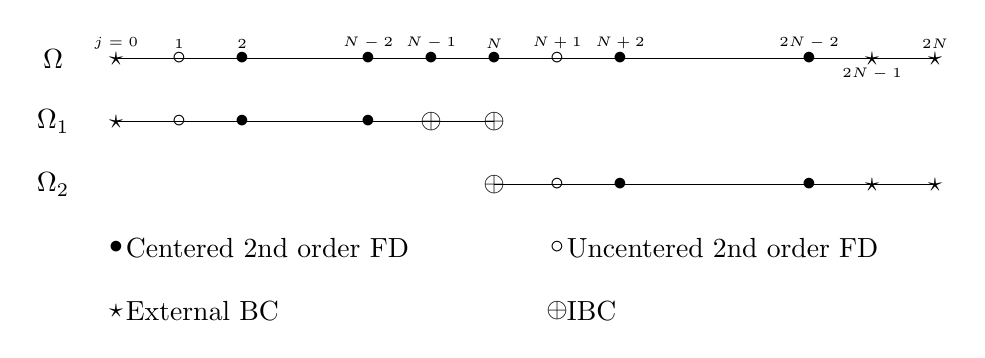
\begin{tikzpicture}[scale = .8]
	\coordinate (Alabel) at (-1,3);
	\coordinate (Aa) at (0,3);
	\coordinate (Ab) at (1,3);
	\coordinate (Ac) at (2,3);
	\coordinate (Ad) at (4,3);	
	\coordinate (Ae) at (5,3);	
	\coordinate (Af) at (6,3);	
	\coordinate (Ag) at (7,3);	
	\coordinate (Ah) at (8,3);	
	\coordinate (Ai) at (11,3);
	\coordinate (Aj) at (12,3);
	\coordinate (Ak) at (13,3);
	
	\draw (Aa) -- (Ak);
	\draw (Alabel) node {$\Omega$}; 
	\draw (Aa) node[label] {$j=0$};
	\draw (Ab) node[label] {$1$};
	\draw (Ac) node[label] {$2$};
	\draw (Ad) node[label] {$N-2$};
	\draw (Ae) node[label] {$N-1$};
	\draw (Af) node[label] {$N$};
	\draw (Ag) node[label] {$N+1$};
	\draw (Ah) node[label] {$N+2$};
	\draw (Ai) node[label] {$2N-2$};
	\draw (Aj) node[below,font=\tiny] {$2N-1$};
	\draw (Ak) node[label] {$2N$};
		
	\draw (Aa) node {$\star$};
	\draw (Ab) node {$\circ$};
	\draw (Aj) node {$\star$};
	\draw (Ak) node {$\star$};
	
	\draw (Ac) node{$\bullet$};
	\draw (Ad) node {$\bullet$};
	\draw (Ae) node {$\bullet$};
	\draw (Af) node{$\bullet$};	
	\draw (Ag) node{$\circ$};
	\draw (Ah) node {$\bullet$};
	\draw (Ai) node {$\bullet$};


	\coordinate (Blabel) at (-1,2);	
	\coordinate (Ba) at (0,2);
	\coordinate (Bb) at (1,2);
	\coordinate (Bc) at (2,2);
	\coordinate (Bd) at (4,2);	
	\coordinate (Be) at (5,2);	
	\coordinate (Bf) at (6,2);	

	\draw (Ba) -- (Bf); 
	
	\draw (Blabel) node {$\Omega_1$}; 
	\draw (Ba) node {$\star$};
	\draw (Bb) node {$\circ$};
	
	\draw (Bc) node {$\bullet$};
	\draw (Bd) node {$\bullet$};
	
	\draw (Be) node {$\oplus$};
	\draw (Bf) node {$\oplus$};	
	
	\coordinate (Clabel) at (-1,1);	
	\coordinate (Cf) at (6,1);	
	\coordinate (Cg) at (7,1);	
	\coordinate (Ch) at (8,1);	
	\coordinate (Ci) at (11,1);
	\coordinate (Cj) at (12,1);
	\coordinate (Ck) at (13,1);
		
	\draw (Cf) -- (Ck); 
	\draw (Clabel) node {$\Omega_2$}; 
	\draw (Cf) node{$\oplus$};
	\draw (Cg) node{$\circ$};
	\draw (Ch) node{$\bullet$};	
	\draw (Ci) node{$\bullet$};	
	\draw (Cj) node {$\star$};
	\draw (Ck) node{$\star$};
	
	%% Legend
	\draw (0,0) node {$\bullet$} node[right] {Centered 2nd order FD};
	\draw (7,0) node {$\circ$} node[right] {Uncentered 2nd order FD};
	\draw (0,-1) node {$\star$} node[right] {External BC};
    \draw (7,-1) node {$\oplus$} node[right] {IBC};
	
\end{tikzpicture}
\captionof{figure}{Scheme indicating the discretization imposed to each point in the monodomain and the DDM problems \label{fig:discretizations}}
\endgroup


\subsection{Corrections for the approximate IBCs}

\indent When using approximate IBCs in \replaced[id=2017]{a Schwarz method}{the SWR}, one should guarantee that the converged solutions $u^*$ satisfy the same equation as the solution $u_{ref}$ of the monodomain problem. Nevertheless, one can easily see that, in the convergence, the solution $u^*$ does not satisfy the discrete equation \eqref{eq:FDdiscretization} on the points where the IBCs are imposed (the poins $x_{N-1},x_N \in \Omega_1$ and $x_N \in \Omega_2$). 

\indent As pointed out by \cite{Gander2001}, a finite difference discretization of the IBCs requires a special treatment to be consistent with the monodomain discretization. Therefore, we will formulate modified IBCs \deleted[id=2017]{for the optimized SWR} in order to avoid this problem:

\begin{equation}
	\label{eq:correctedTBC}
    \begin{gathered}
        \Theta_1^{c}(u_2^{k+1}) + \theta_1 = \Theta_1^{c}(u_1^{k}) + \theta_1' \\
        \Theta_2^{c}(u_1^{k+1}) + \theta_2 = \Theta_2^{c}(u_2^{k}) + \theta_2' \\
        \Theta_3^{c}(u_1^{k+1}) + \theta_3 = \Theta_3^{c}(u_2^{k}) + \theta_3'
    \end{gathered}
\end{equation}

\noindent with $\theta_i, \theta_i'$ given by

\begin{gather*}
    \theta_1 = \Delta x c \frac{u_{2,N+1}^{k+1} - 2u_{2,N}^{k+1} + u_{1,N-1}^{k}}{\Delta x^2} + c^2\frac{\Delta x}{\Delta t} \left( u_{2,N}^{k+1} - \alpha_{2,N} \right)\\
    \theta_1' = - c^2\frac{\Delta x}{\Delta t} \left( u_{1,N}^{k} - \alpha_{1,N} \right)
\end{gather*}

\begin{equation*}
\begin{gathered}
    \theta_2 = \frac{\Delta x}{\Delta t} c^2 \left(u_{1,N}^{k+1} - \alpha_{1,N}\right) \\
    \theta_2' = -\frac{\Delta x}{\Delta t} c^2 \left(u_{2,N}^{k} - \alpha_{2,N}\right)
\end{gathered}
\end{equation*}

\begin{equation*}
\begin{gathered}
    \theta_3  = 2\frac{\Delta x}{\Delta t} \left[-\Delta x \left(u_{1,N-1}^{k+1} - \alpha_{1,N-1} \right) - c \left(u_{1,N}^{k+1} - \alpha_{1,N}  \right) \right] \\  + \Delta x \frac{u_{1,N-3}^{k+1} - 2u_{1,N-2}^{k+1} + u_{1,N-1}^{k+1}}{\Delta x^2} \\
    \theta_3' = 0
\end{gathered}
\end{equation*}

\indent It is straightforward to verify that the DDM problem with these modifications in the IBCs insure that the converged solution $u^*$ satisfies, in every point, the same discrete equations as the solution $u^{ref}$ of the monodomain problem \eqref{eq:problemMonodomain}.

\indent In addition, we notice that all the modification terms $\theta_i,\theta_i', \ i = 1,2,3$, are of order $O(\Delta x)$ (they are composed of discrete versions of time derivatives and second spatial derivatives multiplied by $\Delta x$). It is essential to insure that these terms are small, for the consistency with the approximate IBCs $\Theta_i$ to be fulfilled.

\section{Numerical tests for optimizing the IBCs (speed of convergence)}
\label{sec:optim}

\indent Our objective now is to optimize the IBCs in the sense of minimizing the number of iterations of our method until the convergence. We  perform a very large set of tests in order to find the coefficient $c$ \deleted[id=2017]{(which defines the operators based a constant polynomial approximation for the TBCs)} that provide the fastest convergence. To start with, we make this study with fixed time step and space step, in order to analyze exclusively the influence of the coefficient.

\indent As we are interested in the speed with which the solution of the DDM method converges to the reference solution, the criteria of convergence used is

\begin{equation*}
%\label{eq:criteriaConvergence}
	e^{\Omega,k} \leq \epsilon
\end{equation*}

\noindent with $\epsilon = 10^{-9}$ and 

\begin{equation*}
	e^{\Omega,k} = ||u_{ref,N} - u^{k}_N||_2 = \sqrt{\Delta x \left[ \sum_{j=0}^N{\left(u_{ref,j} - u^{k}_{1,j}\right)^2 } + \sum_{j=N}^{2N}{\left(u_{ref,j} - u^{k}_{2,j}\right)^2 } \right] }
\end{equation*}
 
\indent \deleted[id=2017]{In order to simplify the tests and avoid expensive computations, we will always consider $c_L = c_R = c$ in this optimization.}The range of tested coefficients is $[-10.0, 20.0]$ (chosen after initial tests to identify a proper interval), with a step equal to  $0.1$ between them (or even smaller, up to $0.005$, in the regions near the optimal coefficients), and the maximal number of iterations is set to 100.

\subsection{Test varying the initial time step and the interface position}

\indent As said above, in the first set of tests we consider a fixed time step $\Delta t = 20/2560 = 0.0078125$ and a fixed mesh size $\Delta x = 12/500 = 0.024$. Moreover, we consider two subsets of tests, in order to study the speed of convergence with different initial conditions and different sizes of the subdomains:

\begin{enumerate}
	\item Tests varying the initial time step $t_0$, with the interface in the center of the monodomain $\Omega = [-6,6]$;
	\item Tests varying the position of the interface ($x_{interface} = -a + \alpha (b-a)$, where $b = -a = 6$ and $0 < \alpha < 1$), for a fixed initial time $t_0 = 0.78125$.
\end{enumerate}

\indent In all the cases, the reference solution $u^{ref}$ is the solution of the monodomain problem \eqref{eq:problemMonodomain}.

\indent The results are summarized in Figure \ref{fig:optimVarT0Interface}, with the number of iterations plotted as function of the coefficient $c$ (for the positive coefficients). We can see a very similar behavior of all the curves, with two minima whose position do not depend on $t_0$ and $\alpha$ (approximately, $c = 0.20$ and $c=4.5$). For $c<0$, the curves are very similar, with two minima located at $c = -0.10$ and $c = -1.35$, approximately. Moreover, the minima closest to zero ($c=-0.10$ and $c = 0.20$) are both associated with very discontinuous peaks, while the other two minima are associated with smoother curves. A detail of the curves around each positive minima are shown in Figures \ref{fig:optimVarT0PDetail} - \ref{fig:optimVarT0PDetail2} and \ref{fig:optimVarInterfacePDetail} - \ref{fig:optimVarInterfacePDetail2}. Finally, we remark that, for some curves, the minimal number of iterations is associated with the coefficients closest to zero, and, for other ones, to the other minimum, but the minimal number of iterations are very similar (between 5 and 7).

\begingroup
\addtocounter{figure}{1}
\noindent
\begin{minipage}[t]{.5\linewidth}
\begin{center}
	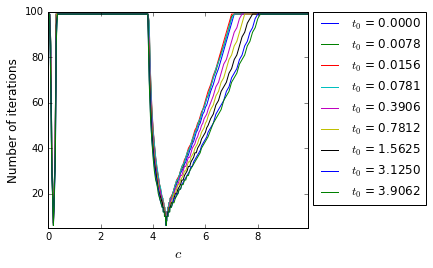
\includegraphics[scale=.375]{Fig3a.png}
	\captionof{subfigure}{General view (for a fixed interface and different values of $t_0$)}
\end{center}
\end{minipage}
\begin{minipage}[t]{.5\linewidth}
\begin{center}
	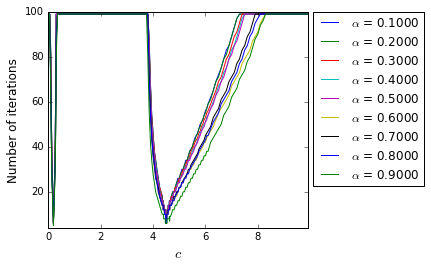
\includegraphics[scale=.375]{Fig3b.png}
	\captionof{subfigure}{General view (for a fixed $t_0$ and different positions of the interface)}
\end{center}
\end{minipage}
\begin{minipage}[t]{.5\linewidth}
\begin{center}
	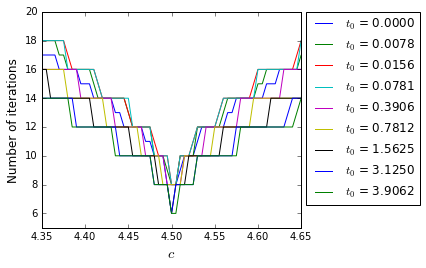
\includegraphics[scale=.375]{Fig3c.png}
	\captionof{subfigure}{Detail around one of the optimal coefficients (for a fixed interface and different values of $t_0$) \label{fig:optimVarT0PDetail} }
\end{center}
\end{minipage}
\begin{minipage}[t]{.5\linewidth}
\begin{center}
	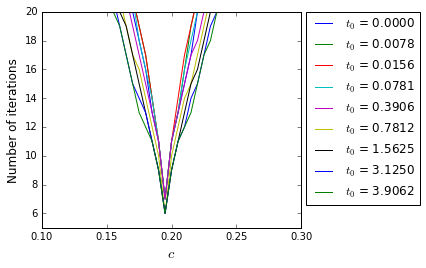
\includegraphics[scale=.375]{Fig3d.png}
	\captionof{subfigure}{Detail around the other optimal positive coefficient (for a fixed interface and different values of $t_0$) \label{fig:optimVarT0PDetail2}}
\end{center}
\end{minipage}
\begin{minipage}[t]{.5\linewidth}
\begin{center}
	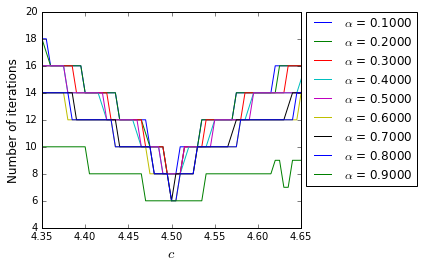
\includegraphics[scale=.375]{Fig3e.png}
	\captionof{subfigure}{Detail around one of the optimal coefficients (for a fixed $t_0$ and different positions of the interface) \label{fig:optimVarInterfacePDetail}  }
\end{center}
\end{minipage}
\begin{minipage}[t]{.5\linewidth}
\begin{center}
	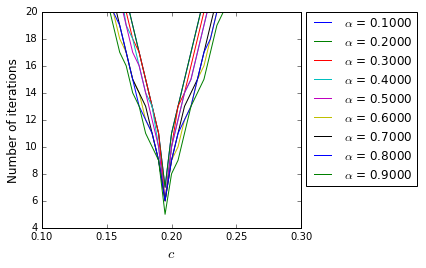
\includegraphics[scale=.375]{Fig3f.png}
	\captionof{subfigure}{Detail around the other optimal positive coefficient  (for a fixed $t_0$ and different positions of the interface) \label{fig:optimVarInterfacePDetail2}}
\end{center}
\end{minipage}
\addtocounter{figure}{-1}
	\captionof{figure}{Number of iterations until the convergence as function of the coefficient of the TBC, in the case of positive coefficients \label{fig:optimVarT0Interface}}
\endgroup

\indent Figure \ref{fig:errorEvolution} shows the evolution of the error, as function of the iterations, for the five positive coefficients $c$ that gave the fastest convergences, for a fixed initial instant and a fixed position of the interface. For other values of $t_0$ and $\alpha$ this graph is similar, concerning the number of iterations and the fact that the convergence is more regular for the coefficients closest to zero, compared to the other optimal coefficients.

\begingroup
\begin{center}
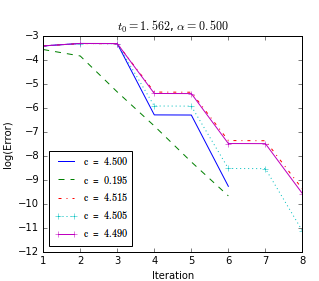
\includegraphics[scale=.5]{Fig4.png}
\captionof{figure}{Error evolution with the iterations for the fastest results \label{fig:errorEvolution}}
\end{center}
\endgroup

\subsection{Tests varying $\Delta t$ and $\Delta x$}

\indent After verifying that the method behaves similarly for \replaced[id=1010]{several initial conditions}{ every initial condition} (\emph{i.e.}, \replaced[id=1010]{for several values of}{ every} $t_0$) and \replaced[id=1010]{various}{ every} positions of the interface, now we keep these parameters fixed ($t_0 = 0$ and $\alpha = 0.5$) and make new tests with different values of $\Delta t$ (with fixed $\Delta x = 12/250$) and different values of $\Delta x$ (with fixed $\Delta t = 0.02$).

\indent The number of iterations as functions of the coefficient, for some of the tests, are shown in Figure \ref{fig:niterxCoefVarDtDx}, in the case of positive coefficients. The results for negative coefficients are similar.

\indent Figure \ref{fig:optimalCoefVarDxDtCorrectN} presents the optimal positive coefficient for each $\Delta t$ or $\Delta x$ (for one fixed value for the other coefficient). Considering the observation we did before about the similar results (\emph{i.e.} the number of iterations until the convergence) for the four optimal coefficients, we only took into account, for the construction of this curve, the positive minimum farther from zero: it was done because, as shown in Figure \ref{fig:niterxCoefVarDtDx}, these minima have a strong dependency on $\Delta t$ or $\Delta x$, and we will seek to study this relation.

\begingroup
\begin{minipage}{.5\linewidth}
\begin{center}
	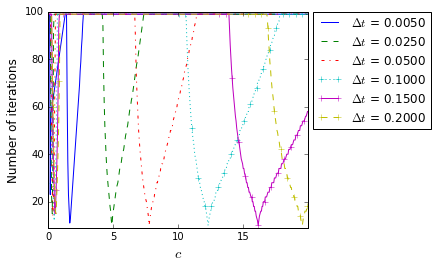
\includegraphics[scale=.375]{Fig5a.png}
\captionof{subfigure}{Fixed $\Delta x = \frac{12}{250}$}
\end{center}
\end{minipage}
\begin{minipage}{.5\linewidth}
\begin{center}
	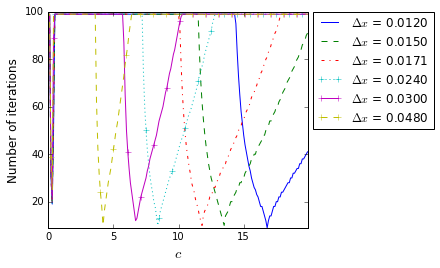
\includegraphics[scale=.375]{Fig5b.png}
\captionof{subfigure}{Fixed $\Delta t = 0.02$}
\end{center}
\end{minipage}
\captionof{figure}{Number of iterations until the convergence as function of the coefficient of the TBC (for positive coefficients)  \label{fig:niterxCoefVarDtDx}}
\endgroup


\begingroup
\begin{minipage}[t]{.5\linewidth}
	\includegraphics[scale=.4]{{Fig6a.png}}
	\captionof{subfigure}{Fixed $\Delta x = \frac{12}{250}$ }
\end{minipage}
\hfill
\begin{minipage}[t]{.5\linewidth}
	\includegraphics[scale=.4]{{Fig6b.png}}
	\captionof{subfigure}{Fixed $\Delta t = 0.02$ }
\end{minipage}
	\captionof{figure}{Optimal coefficients as function of the time step and the space step 	\label{fig:optimalCoefVarDxDtCorrectN}}
\endgroup

\indent Figure \ref{fig:optimalCoefVarDxDtCorrectN} suggests a dependence of the optimal coefficient on $(\Delta t)^\nu$ and $(\Delta x)^\eta$, with $0 \leq \nu \leq 1$ and $\eta < 0$. In fact, performing some regressions with $\Delta t $ or $\Delta x$ fixed, we conclude that $\nu = \frac{2}{3}$ and $\eta = -1$ provide really well-fitted regression curves (with the coefficients of determination $R^2$ bigger than 0.99), both for the negative and the positive coefficients (although each one of these cases correspond to different curves). Therefore, we seek to model a function

\begin{equation*}
	c_{opt}(\Delta t, \Delta x) = \kappa + \alpha (\Delta t)^{\frac{2}{3}} + \beta \frac{1}{\Delta x} + \gamma   \frac{(\Delta t)^{\frac{2}{3}}}{\Delta x}
\end{equation*}

\indent A regression using the corners of the rectangle $[0.001,0.1]\times[12/100,12/1000]$ and fifteen inner points gives the surfaces

\begin{gather}
	c_{opt}^+(\Delta t, \Delta x) = 0.0775 -0.3353 (\Delta t)^{\frac{2}{3}} - 0.0012 \frac{1}{\Delta x} + 2.7407   \frac{(\Delta t)^{\frac{2}{3}}}{\Delta x} 	\label{eq:regression2DPos} \\
	c_{opt}^-(\Delta t, \Delta x) = -0.0583 -1.5024 (\Delta t)^{\frac{2}{3}} - 0.0006 \frac{1}{\Delta x} -0.7287  \frac{(\Delta t)^{\frac{2}{3}}}{\Delta x} 	\label{eq:regression2DNeg}
\end{gather}

\noindent respectively for the positive and the negative optimal coefficients. The coefficients of determination of each regression are $R^{2,+} = 0.9999894$ are $R^{2,-} = 0.9998993$, showing an excellent representation.

\indent In order to validate the expressions \eqref{eq:regression2DPos} and \eqref{eq:regression2DNeg}, we used them to compute the optimal coefficients for several points $(\Delta t, \Delta x)$, with $\Delta t \in [0.0005,0.3]$ and $\Delta x \in \left[ 12/5000,12/50\right]$. For almost all the points in the considered domain, the computed optimal coefficient provides a fast convergence to the monodomain solution, with less than 20 iterations, what is also observed in the case of the negative coefficients. The numbers of iterations observed are not always the smallest ones that we could find (cf. Figures \ref{fig:optimVarT0Interface} to \ref{fig:niterxCoefVarDtDx}), because the expressions \eqref{eq:regression2DPos} and \eqref{eq:regression2DNeg} are regressions constructed from optimal coefficients obtained among a discrete set of possible values. Nevertheless, they give a very good approximation for the optimal $c$ for each $(\Delta t, \Delta x)$, and one could search around a small region around the computed $c_{opt}$ to obtain an even faster convergence.

%\begingroup
%	\centering
%	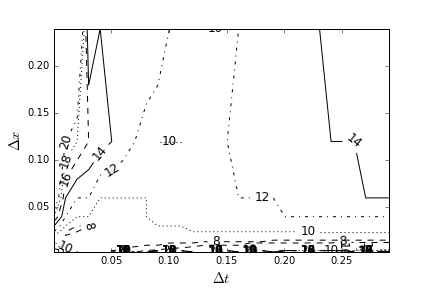
\includegraphics[scale=.6]{figures/FinalFigures/contourValidationP.png}
%\captionof{figure}{Contour lines showing the number of iterations until the convergence, when using the regressions surfaces for obtaining $c_{opt}^+(\Delta t, \Delta x)$ \label{fig:regressionValidation}}.
%\endgroup
 
\indent The results presented in this section show that the DDM proposed here \deleted[id=2017]{, consisting in an optimized SWR with our proposed interface conditions,}is able to provide a fast convergence toward the solution of the monodomain problem. Furthermore, using the corrected IBCs \eqref{eq:correctedTBC}, this convergence is exact. Therefore, we reached our goals of solving the dispersion equation in a finite domain divided in two subdomains.

\indent Moreover, the results of the optimization tests are very satisfying regarding a more general application of our method. Firstly, for fixed spatial and temporal discretizations, we obtained optimal coefficients for the method independently of the initial solution and the size of the subdomains (\emph{i.e.}, independently of the initial instant and the position of the interface). Secondly, we obtained good regression expressions for the optimal coefficient as function of $\Delta t$ and $\Delta x$, which could allow the application of the model, with fast convergence, in other computational frameworks.













